\chapter{Theory}
\section{Modelling of light propagation in tissue}
Photon that propagates through tissue can be described by the radiative transport equation, and in the case of low absorption, can be approximated as a diffusive process \cite{Ishimaru1978,rossum_99_1}. The derivation of the photon diffusion equation from the transport equation has its origin in nuclear transport theory \cite{Case1967}. For now it can be simply stated that in a homogenous media with low absorption and high scattering, the photon fluence rate $\Phi({\bf r},t) \ (W/cm^{2})$ (not fluence which is in ($\rm{J/m}^{2}$)) obeys the diffusion equation:
\begin{equation}
\label{DEtime}
\nabla\cdot ( D({\bf r}) \nabla \Phi({\bf r},t)) - v\mu_a({\bf r}) \Phi({\bf r},t) + v S({\bf r},t) = \frac{\partial \Phi({\bf r},t)}{\partial t}
\end{equation}
\noindent
where ${\bf r}$ is the position vector, $t$ is time, $v$ is the speed of light in the medium, $\mu_a({\bf r})\ (\rm{cm^{-1}})$ is the absorption coefficient, $D(\vec{r})=\frac{v}{3(\mu_a(\bf{r})+\mu_s^{\prime}({\bf r}))}$ is the diffusion coefficient constant where $\mu_s'({\bf r}) (\rm{cm^{-1}})$ is the reduced scattering coefficient, and $S({\bf r},t)\ (\rm{W/cm^{3}})$ is the source term. \\
In the near-infrared (NIR) wavelength range in the human breast $\mu_a\sim 0.05\,\rm{cm^2}$ and $\mu_s^{\prime}\sim 8\,\rm{cm^2}$ In the frequency domain the point light source can be modulated at some angular frequency $\omega$ (which we can model with a delta function) which results in our source and the resulting  signal having a DC and AC component. 
\begin{eqnarray}
\label{AC}
S({\bf r},t) & = & [S_{dc} + S_{ac}e^{-i\omega
  t}]\delta({\bf r}) \\
\label{I_AC}
\Phi({\bf r},t) & = & \Phi({\bf r})_{dc} + \Phi({\bf r})_{ac}e^{-i\omega t}
\end{eqnarray}
\noindent
where  $S_{dc}$ is the DC light intensity, $S_{ac}$ the AC light intensity of the laser source, and \ref{I_AC} is the corresponding fluence rate out of the turbid media. In later chapters, we will be mainly concerned with the diffusion equation in the Frequency-domain (FD). So focusing on just the AC component, the diffusion equation becomes
\begin{equation}
\label{DE}
[-\nabla \cdot D({\bf r}) \nabla + v \mu_a({\bf r})-i\omega]\Phi_{ac}({\bf
  r},\omega)=vS_{ac}\delta({\bf r}).
\end{equation}
\noindent
Now that we have Eqn.~\ref{DE}, we will now solve for this equation analytically for the most common geometries used in our models: infinite, semi-infinite and slab geometries.

\subsection{Analytical Solutions}
In this section we will go over three analytical solutions to the photon diffusion equation. We will solve for the fluence rate $\Phi$ in the infinite, the semi-infinite, and the slab geometries in a homogeneous media. For the infinite medium, we will find the solution by solving the Green's function for the Helmholtz equation. For the semi-infinite and slab problems we will use the method of images after determining the extrapolated boundary condition for the appropriate placement of our sources and sinks.

\subsubsection{Infinite Geometry}
We start with the diffusion equation in the frequency domain (Eqn.~\ref{DE}). Assuming that we are working with homegeneous media, we assume that $D$ is constant. Dividing both sides by $D$ and defining a constant $k_0^2 = \frac{- v\mu_a + i\omega}{D}$, (Eqn.~\ref{DE}) becomes
\begin{equation}
\label{DEHelm}
(\nabla^2+k_0^2)\Phi({\bf r})=-\frac{vS_{AC}}{D}\delta({\bf r})
\end{equation}
\noindent
Here we define ${\bf r}$ the position vector a distance $r$ away from the source. In this form we see that the photon fluence rate $\Phi$ is the Green's function for the Helmholtz equation.
\begin{equation}
\label{greenHelm}
(\nabla^2+k_0^2)G({\bf r})=-\frac{vS_{AC}}{D}\delta({\bf r})
\end{equation}
\noindent
In the infinite medium there are no boundary surfaces so the Green's function is spherically symmetric and depend only on $r={\bf r}$. The Laplace equation in spherical coordinates is then:
\begin{eqnarray}
\label{laplacian}
\nabla^2 & \equiv & \frac{1}{r}\frac{\partial^2}{\partial r^2}r 
+ \frac{1}{r^2\sin^2\theta}\frac{\partial^2}{\partial\phi^2}
+ \frac{1}{r^2\sin\theta}\frac{\partial}
{\partial\theta}\left(\sin\theta\frac{\partial}{\partial\theta}\right)
\nonumber \\
& = & \frac{1}{r}\frac{\partial^2}{\partial r^2}r
\end{eqnarray}
Then Eqn.~\ref{greenHelm} becomes
\begin{equation}
\label{greenHelmLaplace}
\frac{1}{r}\frac{\partial^2}{\partial r^2}rG(r) + k_0^2G(r) 
=-\frac{vS_{AC}}{D}\delta(r)
\end{equation}
\noindent
at every point except at ${\bf r} = 0$ the equation is 
\begin{equation}
\label{greenHelmLaplaceHomog}
\frac{\partial^2}{\partial r^2}[rG(r)] + k_0^2[rG(r)] = 0
\end{equation}
\noindent
for which the solution is 
\begin{equation}
\label{greenHelmLaplaceSoln1}
G(r) = \frac{A e^{ik_0r} + B e^{-ik_0r}}{r} = \frac{A e^{ik_0r}}{r}
\end{equation}
The first term of the Green's function is propagating away from the source while the second term converges, so we will only keep the first term. One could also argue that as we move infinitely away from the source the Green's function needs to go to zero which would mean that $B=0$ by noting that $k_0$ is complex. This leaves us with solving for A for which we go back to equation \ref{greenHelm}. We take a volume integral on both sides in the limit where $r \rightarrow 0$ where the delta function exists.
\begin{equation}
\label{greenHelmdelta}
\lim_{r\rightarrow 0}\int_V[\nabla^2G({\bf r})+k_0^2G({\bf r})]dV =
-\lim_{r\rightarrow 0}\int_V \frac{vS_{AC}}{D}\delta({\bf r})dV =-\frac{vS_{AC}}{D}
\end{equation}
\noindent
Looking at the second term on the LHS in spherical coordinates, we see that it goes to zero
\begin{equation}
\label{greenHelm2nd}
\lim_{r\rightarrow 0}\int_Vk_0^2G({\bf r})dV = \lim_{r\rightarrow
  0}\int\int\int k_0^2\frac{A e^{ik_0r}}{r} r^2\sin\theta d\phi d\theta=0
\end{equation}
For the first term on the LHS , we use Gauss theorem
\begin{eqnarray}
\label{greenHelm1st}
  \lim_{r\rightarrow 0}\int_V\nabla^2G({\bf
    r})dV&=&\lim_{r\rightarrow 0} \int_S (\nabla G) \cdot {\bf dS} =
  \lim_{r\rightarrow 0} \int_S(\nabla\frac{A e^{ik_0r}}{r}) \cdot
  d{\bf S}\nonumber\\  
  &=&\lim_{r\rightarrow 0}\int_S\frac{ik_o A e^{ik_0r}}{r}-\frac{A
    e^{ik_0r}}{r^2}d{\bf S}\nonumber\\
  &=&\lim_{r\rightarrow 0}\int_S[\frac{ik_o A e^{ik_0r}}{r}-\frac{A
    e^{ik_0r}}{r^2}]r^2\sin\theta d\phi d\theta\nonumber\\
  &=&A\ 4\pi
\end{eqnarray}
\noindent
Plugging this back into equation \ref{greenHelmdelta} gives us $A = \frac{vS_{AC}}{4\pi D}$ and brings us to the well known result:
\begin{equation}
\label{InfiniteSoln1}
G({\bf r}) = \frac{vS_{AC}}{4\pi D}\frac{e^{ik_or}}{r}
\end{equation}

\subsubsection{Semi-infinite Geometry}
Now that we have the solution to the infinite media it is easy to solve for the semi-infinite geometry. One assumption that will be made here is that there will be an extrapolated zero boundary located at some distance $\ell$ away from the air-diffusive media interface ($z=0$). At this boundary the fluence rate is set to be $\phi=0$ as shown in figure \ref{semiinf}. What this boundary is and the value of $\ell$ will be addressed later in this section. 
To find the solution, we take a page from an undergrad electrostatics textbook and use the method of images. If there is a source some distance $\ell + z_s$ away from the boundary, we can place a sink the same distance away from the boundary so that the net fluence at the boundary between them is zero. The solution is then a Green's function for the infinite media of the source and the negative image source given by
\begin{equation}
\label{semisoln}
G(\rho_s,z_s;\rho,z) = \frac{vS_{ac}}{4\pi D} \left( \frac{exp[ikr_+]}{r_+} 
- \frac{exp[ikr_-]}{r_-} \right) \nonumber
\end{equation}
\begin{eqnarray}
\label{ext_both}
r_{+} = & \sqrt{(\rho-\rho_s)^2+(z-z_{+})^2} \nonumber \\
r_{-} = & \sqrt{(\rho-\rho_s)^2+(z-z_{-})^2}
\end{eqnarray}
\noindent
where $z_+=z_s$ is the position of the source and $z_-=-2\ell-z_s$ is the position of our image source. Note that the source is not placed on the surface of the turbid media and air interface (where a tip of the fiber might be placed) The photons coming out of the source fiber is initially pointed in towards the media and has a survival probability given by an exponential decay before experiencing a scattering or absorption event \ref{Ishimaru1978,Arridge1999}.
\noindent
\begin{equation}
\label{scatterprob}
  P(z) = e^{-(\mu_s'+\mu_a)z} \approx e^{-\mu_s'z}
\end{equation}
\noindent
Then one can find the mean depth of penetration by the photon by taking the expected value. First we normalize the distribution to allow for one scattering event.
\noindent
\begin{equation}
  1 = \int_o^\infty C e^{-\mu_s'z}dz = C \frac{1}{\mu_s'} \implies C = \mu_s'
\end{equation}  
\noindent
Now the expected value or mean depth the photon travels before being scattered or absorbed.
\noindent
\begin{equation}
  z_+ = <z> = \int_o^\infty Cz e^{-\mu_s'z}dz =\int_o^\infty \mu_s'z
  e^{-\mu_s'z}dz = \frac{1}{\mu_s'} 
\end{equation}
\noindent
We have solved the above equation using integration of parts, and determined that the isotropic source position located $1/ \mu_s'$ inside of the media.
\noindent
\begin{figure}[h]
\centering
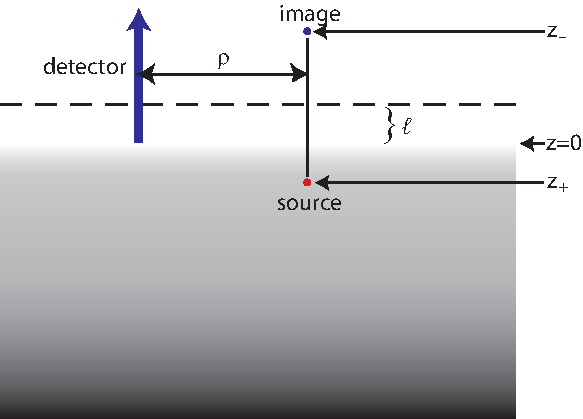
\includegraphics[width=11cm]{./figures/2_Theory/semiinfinite.pdf}
\caption{The semi-infinite case where the image method is used to find the solution.}
\label{semiinf}
\end{figure}

\subsubsection{Slab Geometry}
The solution for the slab geometry is just an expansion on the solution for the semi-infinite case. We use the method of images again. This time there is a second boundary located on the bottom, and we again make the assumption that $\Phi=0$ some distance $\ell$ away from the air-diffuse media interface on the bottom $z=L$ as well. As in the semi-infinite case, we add an image charge above the top boundary. But now we need to add another image below the bottom boundary to cancel our source on that side as well. In fact, we need to cancel the first image on the top across the bottom boundary too.
Now we need to account for these images with more images above the top boundary again!! Now you see that we can do this again and again... We start to see a pattern in the position of these sources and we can write the Green's function for the original source and all these images as an infinite sum:
\begin{figure}[h]
\begin{center}
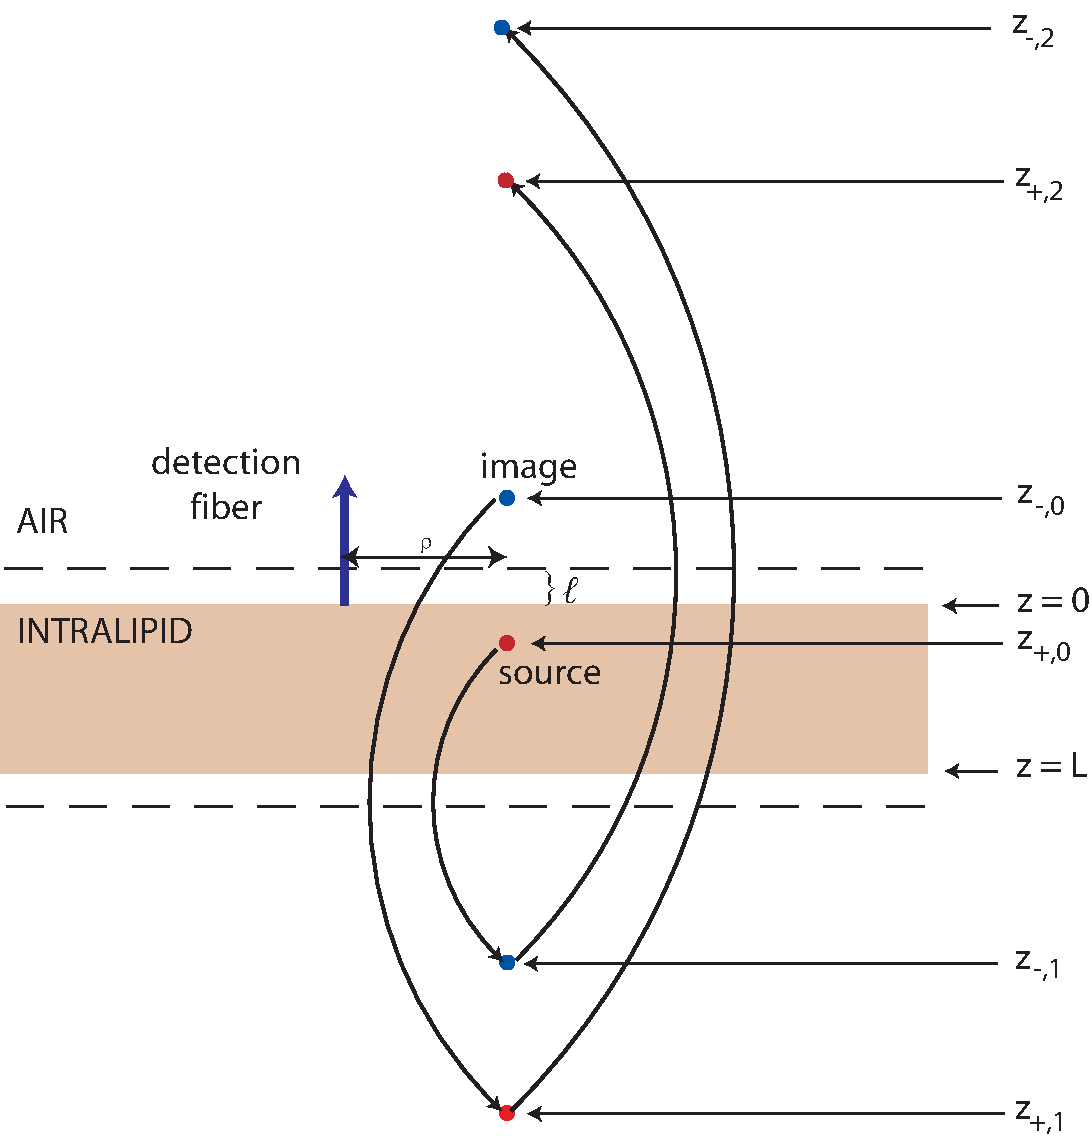
\includegraphics[width=10cm]{./figures/2_Theory/slab3.pdf}
\caption{The slab case where the image method is used again to find  the solution. This time since there are two boundaries, we have to sum over a larger number of source and sink images.}
\label{slab}
\end{center}
\end{figure}
\begin{equation}
G(\rho_s,z_s;\rho,z) = \frac{vS_{AC}}{4\pi D} \sum_{m=-\infty}^{m=\infty} 
\left\{ \frac{exp[ikr_{+,m}]}{r_{+,m}} - \frac{exp[ikr_{-,m}]}{r_{-,m}} \right\} \notag
\end{equation}
\begin{eqnarray}
\label{ext_both}
r_{+,m} = & \sqrt{(\rho-\rho_s)^2+(z-z_{+,m})^2} \notag \\
r_{-,m} = & \sqrt{(\rho-\rho_s)^2+(z-z_{-,m})^2}
\end{eqnarray}
\noindent
where $z_{+,m}=2m(L+2\ell)+z_s$, $z_{-,m}=2m(L+2\ell)-2\ell-z_s$, $m=0,\pm 1, \pm 2, ...$, and $L$ is the thickness of the slab. For the semi-infinite geometry, only the $m=0$ term is used. 

\subsection{Boundary Conditions}
In this section we will determine the value of $\ell$ that we used before for our semi-infinite and slab solutions \cite{haskell_94_1}. We start by defining the radiance ($\rm{W/m^2sr^1}$), which measures the amount of light passes through a given area within some solid angle in a specific direction. Integrating the radiance over all possible angles will give us the fluence rate that we've been using thus far. 
\begin{eqnarray}
\Phi({\bf r}) &=& \int\int_{4\pi} d\Omega \ L({\bf r},{\bf s})\\
{\bf j}({\bf r}) &=& \int\int_{4\pi} d\Omega \ L({\bf r},{\bf s}) \ {\bf s}
\end{eqnarray}
In the diffusion approximation, the radiance can be approximated by an isotropic fluence rate term plus an additional term for some small directional flux pointing along ${\bf s}$:
\begin{equation}
\label{Radiance}
L({\bf r},{\bf s}) = \frac{1}{4\pi} [ \Phi({\bf r}) + 3 {\bf j}({\bf
  r}) \cdot {\bf s}] \ .
\end{equation}
\begin{figure}[h]
\centering
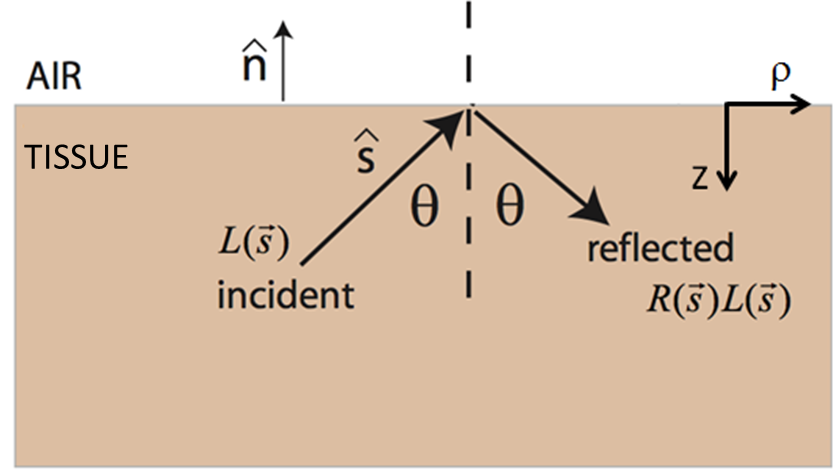
\includegraphics[width=8cm]{./figures/2_Theory/BoundaryReflect.png}
\caption{At the boundary, some of the incident light is Fresnel reflected back into the media due to index mismatch. This reflected light accounts for all of the light that is diffusing inwards towards the media at the boundary.}
\label{BoundaryReflect}
\end{figure}
Since we are interested in taking noninvasive measurements, we will look at the radiance at the air-tissue boundary. If ${\bf n}$ is the outward normal the tissue surface and ${\bf s}$ gives us the direction of the light propagation, then the fluence rate of the light exiting and entering the tissue is given by integrating $L({\bf s}) ({\bf s} \cdot {\bf n})$ over all outward directions and integrating  $L({\bf s}) ({\bf s} \cdot {- \bf n})$ over all inward directions
respectively. Air is not a scattering medium so there is no light entering the tissue from the boundary with the exception of the Fresnel reflected light of the outgoing light due to the index mismatch at the boundary. If $R({\bf \theta})$ is the Fresnel reflection coefficient for unpolarized light, then
\begin{equation}
\label{bc1}
\int\int_{{\bf s} \cdot {\bf n} > 0} R({\bf s}) L({\bf s}) ({\bf s} \cdot {\bf n}) d\Omega =
\int\int_{{\bf s} \cdot {\bf n} < 0} L({\bf s}) ({\bf s} \cdot {- \bf
  n}) d\Omega \ .
\end{equation}
\begin{equation}
\label{bc2}
\frac{1}{4\pi}\int\int_{{\bf s} \cdot {\bf n} > 0} R({\bf s}) [ \Phi({\bf r}) + 3 {\bf j}({\bf r}) \cdot {\bf s}] ({\bf s} \cdot {\bf n}) d\Omega = \frac{1}{4\pi} \int\int_{{\bf s} \cdot {\bf n} < 0} [ \Phi({\bf r}) + 3 {\bf j}({\bf r}) \cdot {\bf s}] ({\bf s} \cdot {-\bf n}) d\Omega \ .
\end{equation}
Changing into spherical coordinates, ${\bf s}\cdot{\bf n}=\cos\theta$ and ${\bf j}\cdot{\bf n}=j_z\cos\theta$, the integral
on the RHS then becomes
\begin{eqnarray}
\label{bc3}
\frac{1}{4\pi}\int\int_{{\bf s} \cdot {-\bf n}} [-\Phi\cos\theta + 3j_z\cos^2\theta]\sin\theta d \phi d\theta &=& \frac{1}{4}\int_{\pi/2}^{\pi} [-\Phi\cos\theta + 3j_z\cos^2\theta]\sin\theta d\theta \nonumber\\ 
&=&\frac{1}{2}\int_{0}^{-1} [\Phi u - 3j_zu^2] du \notag \\
&=&\frac{\Phi}{4}+\frac{j_z}{2}
\end{eqnarray}
\noindent
where I have used $u=\cos\theta$ substitution to get the second line. Similarly, the integral on the LHS becomes
\begin{eqnarray}
\label{bc4}
\frac{1}{4\pi}\int\int_{{\bf s} \cdot {\bf n}} R({\bf s})[\Phi\cos\theta -
3j_z\cos^2\theta]\sin\theta d \phi d\theta &=&  \frac{1}{4}\int_{0}^{\pi/2}
 R({\bf \theta})[\Phi\cos\theta - 3j_z\cos^2\theta]\sin\theta d\theta \nonumber\\
&=& \frac{1}{4}\Phi\int_{0}^{\pi/2}2R({\bf \theta})\cos\theta\sin\theta
d\theta - \nonumber \\
& & \frac{1}{2} j_z\int_{0}^{\pi/2}3R({\bf \theta})\cos^2\theta\sin\theta d\theta \nonumber \\
&=&\frac{\Phi}{4}R_\Phi-\frac{j_z}{2}R_j
\end{eqnarray}
\noindent
where we have defined
\begin{equation}
\label{Rj}
R_j = \int_0^{\pi/2} 2 sin \theta \ cos^2 \theta \ R(\theta) \ d\theta
\end{equation}
\begin{equation}
\label{Ru}
R_{\Phi} = \int_0^{\pi/2} 3 sin \theta \ cos \theta \ R(\theta) \ d\theta
\end{equation}
\noindent
and $R(\theta)$ are the Fresnel Reflection coefficients for which I give the expression below for unpolarized light.
\begin{equation}
R(\theta) = \left\{ \begin{array}{ll}
    \frac{1}{2}(\frac{n_{media}\cos\theta'-n_{air}\cos\theta}
                     {n_{media}\cos\theta'+n_{air}\cos\theta})^2 +
 \frac{1}{2}(\frac{n_{media}\cos\theta-n_{air}\cos\theta'}
                     {n_{media}\cos\theta+n_{air}\cos\theta'})^2 
      & \mbox{when $0 \leq \theta \leq \theta_c$} \\
    1 & \mbox{when $\theta_c \leq \theta \leq \pi /2$ }
    \end{array}
  \right.
\end{equation}
\noindent
Now plugging in Eqn.~\ref{bc3} and \ref{bc4} into equation \ref{bc1} we get
\begin{equation}
\label{bc2}
R_{\Phi}\frac{\Phi}{4} - R_j \frac{j_z}{2} = \frac{\Phi}{4} + \frac{j_z }{2}
\end{equation}
\\
We now introduce the effective reflection coefficient which we will
define as
\begin{equation}
R_{eff} = \frac{R_{\Phi} + R_j}{2 - R_{\Phi} + R_f} \
\end{equation}
\\
which simplifies Eqn.~\ref{bc2} to give us
\begin{equation}
\label{bc3}
R_{eff} \left( \frac{\Phi}{4} - \frac{j_z}{2} \right) = \frac{\Phi}{4} + \frac{j_z}{2} \ .
\end{equation}
\\
which shows us that $R_{eff}$ gives us the fraction of the radiance that is reflected. 

We can also determine the value of $R_{eff}$ experimentally. We start with the obvious statement that the reflectance and transmission accounts for all of the photons
\begin{equation}
  R + T = 1 \ .
\end{equation}
For diffuse media, we can relate the internal and external transmission ($T_{internal}, T_{external}$ based on Snell's law and conservation of energy (Orchard 1969)
\begin{equation}
  T_{internal} = T_{external} /n_{rel}^2
\end{equation}
where $n_{rel} = n_{medium}/n_{air}$ is the relative refractive index. Now we state that
\begin{equation}
\label{refinttoext}
R_{internal} = 1 - (1 - R_{external})/n_{rel}^2
\end{equation}
Egan (1979) \cite{Egan1979} did a power series curve fit to the external reflectance data tabulated by Orchard \cite{Orchard1969} to get
\begin{equation}
R_{external} = 0.440 + 0.710n_{rel} -0.332n_{rel}^2 + 0.0636n_{rel}^3
\end{equation}
From \ref{refintoext} we find that \cite{Sevick2002}
\begin{equation}
\label{exp eff}
R_{eff} = R_{internal} = -1.440n_{rel}^{-2} + 0.710n_{rel}^{-1} + 0.668 + 0.0636n_{rel}
\end{equation}
\noindent
We further simplifiy \ref{bc3} by using a relation known as Fick's rule which draws its name from its similarity to the equation describing ordinary gas diffusion.
\begin{equation}
j_z = -D \nabla \Phi \cdot {\bf z} \ ,
\end{equation}
\noindent
This is actually a basic relation that comes out of the diffusion approximation and comes out during the derivation of the diffusion equation from the radiative transport equation \cite{Case1967} to be covered in a later section. Using this relation, \ref{bc3} becomes
\begin{equation}
\label{bc4}
\Phi + \left[2D \frac{1+R_{eff}}{1-R_{eff}}\right] \nabla \Phi \cdot {\bf n} = 0 \ .
\end{equation}
or
\begin{equation}
\label{BC_DE}
\Phi + \ell\ \nabla \Phi\cdot{\bf n} = 0
\end{equation}
\\
\noindent
where we have replaced the terms inside the square bracket with $\ell$. From here we can use the Extrapolated-Boundary Condition \cite{haskell_94_1,Aronson1993,Aronson1995} which states that the fluence rate drops lienarly to zero at the distance $\ell$ away from the boundary that we have worked out ($\Phi(\rho,z=-\ell) = 0$). Then we have the boundary we need to solve for the semi-infinite and slab geometries we covered earlier in the section.
\vspace{3mm}
Additionally, We can also determine the value of $R_{eff}$ experimentally. We do this by stating that the reflectance and transmission accounts for all of the photons
\begin{equation}
  R + T = 1 \ .
\end{equation}
For diffuse media, we can relate the internal and external transmission ($T_{int}, T_{ext}$ based on Snell's law and conservation of energy (Orchard 1969)
\begin{equation}
  T_{int} = T_{ext} /n_{rel}^2
\end{equation}
where $n_{rel} = n_{medium}/n_{air}$ is the relative refractive index. Now we state that
\begin{equation}
\label{refinttoext}
R_{internal} = 1 - (1 - R_{external})/n_{rel}^2
\end{equation}
Egan (1979) \cite{Egan1979} did a power series curve fit to the external reflectance data tabulated by Orchard \cite{Orchard1969} to get
\begin{equation}
R_{external} = 0.440 + 0.710n_{rel} -0.332n_{rel}^2 + 0.0636n_{rel}^3
\end{equation}
From \ref{refinttoext} we find that \cite{Sevick2002}
\begin{equation}
\label{exp eff}
R_{eff} = R_{internal} = -1.440n_{rel}^{-2} + 0.710n_{rel}^{-1} + 0.668 + 0.0636n_{rel}
\end{equation}
\begin{figure}[h]
\centering
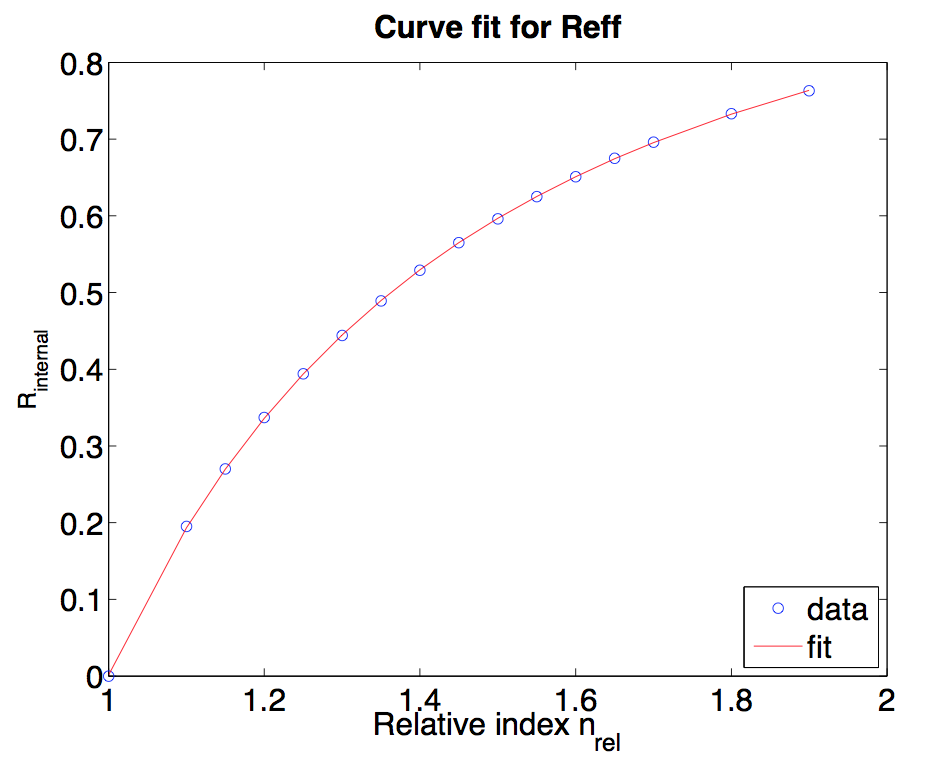
\includegraphics[width=10cm]{./figures/2_Theory/ReflectanceCurveFit.png}
\label{ReflectanceCurveFit}
\caption{A plot showing the tabulated data taken by Orchard fitted with the power series given by Egan.} 
\end{figure}

\section{Reconstruction Methods}
When using DOT to get the optical properties of human tissue, we are trying to solve for $\mua$ and $\musp$ for points in a 3 dimensional space given that we know the light source input and the measured output at some surface for a known geometry. Common reconstruction methods are then divded into two steps: 1) the forward problem and 2) the inverse problem.

The forward problem involves solving for the the fluence of photons at a surface point given that the values of $\mua$ and $\musp$ and information about the input source is given. Solving the inverse problem involves determining the values of $\mua$ and $\musp$ given that the fluence at the boundary is known. This is generally the situation we have in experiments where we have knowledge about the light that we put in and the light that we measure and want to solve for the optical properties inside the media. 

For the forward problem, general approaches can be divided into three groups. There is the analytical methods, numerical methods, and Monte-Carlo (MC) methods from least to most computationally demanding respectively. The analytical method is the fastest and easiest to solve and involve using the Green's function to solve for a given source distribution. The limitations comes from the assumptions it has to make and that the problem is ill-conditioned. Numerical methods are attractive because the minimize the number of assumptions and include techniques such as the Finite Element Method (FEM) and Finite Difference Method (FDM). The Monte-Carlo approach is a stochastic method which models the transport of photons through the tissue and traced through with probability of absorption and scattering events until the photon exits or is absorbed. This is done for a large number of photons $10^6-10^7$ and is very computationally expensive. Of these methods we will look at reconstruction methods from the first two groups.

For linear forward problems we go over two linear inverse problem approaches using an analytic and algebraic approach to be discussed in Sec.~\ref{sec:analytic} and \ref{sec:algebraic}. The advantage of these methods over nonlinear methods are its speed and 




\subsection{Linear Reconstruction Methods}
\label{sec:linearrecon}



\subsection{Linearized integral equations}
\label{subsec:lin_eq}

This research employs linear image reconstruction methods and CW data. In principle, one could also resort to
time-~\cite{patterson_89_1,benaron_93_1,andersson-engels_90_1,jacques_89_1,schmidt_00_2,ntziachristos_98_1}
or frequency-resolved~\cite{gratton_90_1,fishkin_93_1,chance_98_1,pogue_94_1} measurements and nonlinear reconstruction methods~\cite{arridge_99_1,markel_03_2} to obtain a reconstruction of
the target and the chest wall phantom simultaneously; however, these
approaches require more expensive and complex instrumentation, as well
as more time-consuming computational schemes. For our linear approach,
two independent measurements of the transmitted intensity are taken,
one in a homogeneous (reference) slab and the other in a slab with the
target and the chest wall phantom present. We denote these
measurements by $I_0({\bf r}_{\rm d}, {\bf r}_{\rm s})$ and $I({\bf
  r}_{\rm d}, {\bf r}_{\rm s})$, respectively, where ${\bf r}_{\rm d}$
and ${\bf r}_{\rm s}$ are the two-dimensional vectors specifying the
lateral positions of the detector and the source on the respective
surfaces of the tank. In this work, $I_0$ and $I$ are expressed in CCD
counts. These measurements can be related to the medium optical
properties through the relations
%
\begin{equation}
I({\bf r}_{\rm d}, {\bf r}_{\rm s}) =
A({\bf r}_{\rm d})B({\bf r}_{\rm s})G({\bf r}_{\rm d},{\bf r}_{\rm s})
\ , \ \ 
I_0({\bf r}_{\rm d},{\bf r}_{\rm s})=
A({\bf r}_{\rm d})B({\bf r}_{\rm s})G_0({\bf r}_{\rm d},{\bf r}_{\rm
  s}) \ .
\label{eq1}
\end{equation}
%
\noindent
Here $A({\bf r}_{\rm d})$ and $B({\bf r}_{\rm s})$ are unknown
coupling coefficients associated with the source and detection system
which can be excluded from consideration as described below. $G({\bf
  r}_{\rm d}, {\bf r}_{\rm s})$ and $G_0({\bf r}_{\rm d}, {\bf r}_{\rm
  s})$ are the Green's functions for the diffusion equation in the
slab with the inhomogeneities present and in the homogeneous and reference 
slab, respectively. The latter is known
analytically~\cite{markel_04_4}. The two Green's functions are
mathematically related by the Dyson equation. Under the assumption
that the scattering properties of the medium are spatially uniform,
the Dyson equation has the form
%
\begin{equation}
G({\bf r}_{\rm d}, {\bf r}_{\rm s}) = G_0({\bf r}_{\rm d}, {\bf r}_{\rm s}) -
\int_V G_0({\bf r}_{\rm d}, {\bf r}) \delta\alpha({\bf r}) G({\bf r},
{\bf r}_{\rm s})\,d^3r \ .
\label{eq2}
\end{equation}
%
\noindent
Here the integral is taken over the volume of the slab and
$\delta\alpha({\bf r}) = c\left[\mu_{\rm a}({\bf r}) - \mu_{{\rm a}0}
\right]$ is the deviation of the absorption coefficient at a given
point from the background value $c\mu_{{\rm a}0}$, where $c$ is the
average speed of light in the medium.

The procedure of linearization consists of making an approximation to
Eq.~(\ref{eq2}) so as to exclude the unknown function $G({\bf r}, {\bf
  r}_{\rm s})$ from the right-hand side. In the first Rytov
approximation~\cite{schotland_97_1}, Eq.~(\ref{eq2}) is rewritten as
%
\begin{equation}
G({\bf r}_{\rm d}, {\bf r}_{\rm s}) = G_0({\bf r}_{\rm d}, {\bf r}_{\rm s})
\exp\left[ -\int_V \frac{G_0({\bf r}_{\rm d}, {\bf r}) \delta\alpha({\bf r})
G({\bf r}, {\bf r}_{\rm s}) \,d^3r}{G_0({\bf r}_{\rm d}, {\bf r}_{\rm s})}
\right] \ .
\label{eq3}
\end{equation}
%
\noindent
Consequently, we define the data function $\phi({\bf r}_{\rm d}, {\bf
  r}_{\rm s})$ according to
%
\begin{equation}
\phi({\bf r}_{\rm d},{\bf r}_{\rm s})=
-G_0({\bf r}_{\rm d},{\bf r}_{\rm s})
\ln\left[\frac{I({\bf r}_{\rm d},{\bf r}_{\rm s})}
{I_0({\bf r}_{\rm d},{\bf r}_{\rm s})}\right]
\label{eq4}
\end{equation}
%
\noindent
and use Eq.~(\ref{eq3}) to obtain an integral equation of the form
%
\begin{equation}
\int_VG_0({\bf r}_{\rm d}, {\bf r})\delta\alpha({\bf r}) G_0({\bf r},
{\bf r}_{\rm s})\,d^3r = \phi({\bf r}_{\rm d}, {\bf r}_{\rm s}) \ .
\label{eq5}
\end{equation}
%
\noindent
Here the right-hand side contains the measurable data function, and the
left-hand side is an integral transform of the contrast whose kernel
is known analytically. This formulation of the linearized inverse
problem of DOT is standard~\cite{schotland_97_1}. The Green's function
$G_0({\bf r},{\bf r}^{\prime})$, which enters Eq.~(\ref{eq5}), is
defined in Ref.~\cite{markel_04_4}.



\subsection{Analytical Inverse Reconstruction}
\label{sec:Analytic}
This method is described in detail in Ref.~\cite{markel_04_4}.  
Its applications to the slab geometry with experimental data have been
reported in Refs.~\cite{wang_05_1,konecky_08_1}. The method requires
the Fourier transform of the data function $\phi({\bf r}_{\rm d}, {\bf
  r}_{\rm s})$ with respect to both variables. To obtain this Fourier
transform, the data function must be measured over sufficiently large
areas so that the integrals involved (approximated by sums in 
practical implementations) have converged. This requirement translates
into the need for sufficiently large imaging windows that was discussed above.

In our experiments, some data points are strongly affected by the 
presence of the chest wall. The actual source and detector positions for the 
affected data points depend on the separation $d$ between the chest wall and 
the top of the bar target. At the two smallest separations ($d=2\,{\rm cm}$ 
and $5\,{\rm cm}$), contamination of the data function by the chest wall is 
significant. Under these circumstances, two approaches for data analysis are 
natural to consider:

\begin{itemize}
  
\item[(i)] Use all data points available (i.e., in a wide window on
  both sides of the slab). This scheme will include, in some cases,
  data points strongly affected by the presence of the chest wall. In
  this case, the analytical image reconstruction algorithm is applied
  as intended by mathematical design, i.e., without additional
  approximations. However, the strong nonlinearity of the inverse
  problem due to the presence of the chest wall phantom renders the
  underlying first Rytov approximation invalid. This, in turn, results
  in poor-quality reconstructions or inability to reconstruct the
  target at all. From the practical point of view, this approach is
  simply not feasible {\em in vivo} because the data, which are
  collected in our experiment over large windows, are physically
  unavailable in the case of a real chest wall.

\item[(ii)] Truncate the data function by replacing data points, which
  are either deemed as physically unavailable {\em in vivo} or as too
  badly contaminated by the presence of the chest wall, with zeroes.
  This is equivalent to replacing a subset of optical measurements
  obtained in the heterogeneous medium with the respective measurements
  obtained in the homogeneous (reference) medium and is substantially
  different from the approach (i) in which these data points are
  simply not used in reconstruction. The approach (ii) is numerically
  efficient and directly applicable {\em in vivo}. In fact, we will
  demonstrate below that it produces images of reasonable quality,
  i.e., of much better quality than approach (i). However, the
  additional approximation involved in this approach results in the
  appearance of image artifacts that are poorly controlled and may be
  viewed as undesirable.

\end{itemize}

Note that in the numerical implementation of the analytical method, we
have followed closely Ref.~\cite{konecky_08_1} with some minor
modifications. Thus, as in~\cite{konecky_08_1}, we have used the
change of variables $\psi({\bf q}, {\bf p}) = \tilde{\phi}({\bf q} +
{\bf p}, -{\bf p})$, where $\tilde{\phi}({\bf q}_{\rm d}, {\bf q}_{\rm
  s})$ is the Fourier transform of the data function defined in
Eq.~(\ref{eq4}).  Here we use a ``symmetric version'' in which
$\psi({\bf q}, {\bf p}) = \tilde{\phi}({\bf q}/2 + {\bf p}, {\bf q}/2
- {\bf p})$. The variables ${\bf p}$ and ${\bf q}$ were sampled as
follows: ${\bf q}_{ij} = \Delta (i\hat{\bf x} + j\hat{\bf y})$, ${\bf
  p}_{kl} = \Delta (k\hat{\bf x} + l\hat{\bf y})$, where $\Delta =
2\pi/(331\times p)$, $-28\le i,j\le 28$ and $0\le k,l\le 6$. This
corresponds to using $57^2=3249$ ``external'' degrees of freedom and
$7^2=49$ ``internal'' degrees of freedom, where the terminology of
Ref.~\cite{markel_04_4} has been used, or a total of
$49\times3249\simeq1.6\times10^5$ independent Fourier-space data
points. Using these parameters, the necessary computations require
$7\times 10^{9}$ floating point operations. On a single-core Intel
Core 2 Duo processor with a peak performance of 19 GFlops, this
translates to 7 minutes of computation time.


\subsection{Algebraic Method}
\label{sec:Algebraic}
\label{subsec:alg_rec}

Algebraic image reconstruction methods are obtained by discretization
of the volume integral in Eq.~(\ref{eq5}) and computation of the
pseudo-inverse for the obtained system of linearized
equations~\cite{gonatas_95_1}.  This method does not require large
windows and can be used with any data restriction. In terms of the two
approaches (i) and (ii) described in Sec.~\ref{subsec:fourier_rec},
the approach (ii) does not involve, in the case of the algebraic
method, any assumptions about the discarded data points, while, in the
analytical reconstruction method, it is assumed that these data points
are zero.  On the other hand, the algebraic method requires explicit
volume discretization in terms of voxels, while the analytical method
allows one to reconstruct the target on any grid without much
additional effort and is not dependent in any way on volume
discretization.

For the purpose of obtaining algebraic reconstructions, the
reconstructed volume was divided into cubic voxels. The voxel size $h$
was taken to be equal to 8 CCD pixels $p$. Thus, $h=8\times
0.416\,{\rm mm}\simeq 3.3\,{\rm mm}$. The grid consisted of $41\times
41$ voxels in the lateral direction and 17 voxels in the depth
direction. Therefore, the discretized volume was a parallelepiped with
the dimensions $13.6\times 13.6\times 4.3\,{\rm cm}^3$ consisting of
$N=21853$ voxels. This parallelepiped was positioned from each surface
of the slab. The target was situated approximately in the middle of
the discretized volume.

The discretization described above, and the approximation of the
integral in Eq.~(\ref{eq5}) with a Riemann sum, results in a system of
algebraic equations $Ax=b$ where $A_{mn}$ is the $M\times N$ weight
matrix, where $M$ is the number of distinct source-detector pairs, $N$
is the number of voxels, $x_n = \delta\alpha({\bf r}_n) / \alpha_0$ is
the vector of dimensionless contrast $(n=1,\dots,N)$ and $b_m$ is the
$m$-th data point $(m=1,\dots,M)$.  The equations are cast in
dimensionless form by defining a dimensionless Green's functions
according to $\tilde{G}_0({\bf r}, {\bf r}^\prime) = D_0 h G_0({\bf
  r}, {\bf r}^\prime)$, where $D_0$ is the diffusion coefficient in
the Intralipid solution. Then we have:
%
\begin{equation}
A_{mn} = (k_{\rm d} h)^2 \tilde{G}_0({\bf r}_{{\rm d}m}, {\bf r}_n)
\tilde{G}_0({\bf r}_n, {\bf r}_{{\rm s}m}) \ , \ \ 
b_m = -\tilde{G}_0({\bf r}_{{\rm d}m}, {\bf r}_{{\rm s}m})
\ln\left[\frac{I({\bf r}_{{\rm d}m}, {\bf r}_{{\rm s}m})}
{I_0({\bf r}_{{\rm d}m}, {\bf r}_{{\rm s}m})}\right] \ .
\label{eq6}
\end{equation}
%
\noindent
Here ${\bf r}_n$ is the position of the center of the $n$-th voxel
while ${\bf r}_{{\rm d}m}$, ${\bf r}_{{\rm s}m}$ are the detector and
the source positions of the $m$-th data point used in the
reconstruction.

The pseudoinverse solution to the above system of equations is defined
as the unique solution to the system $(A^*A + \lambda^2 I)x = A^*b$,
where $\lambda$ is the regularization parameter and $I$ is the
identity matrix. In our experiments, the number of measurements $M$ is
much larger than the number of voxels $N$ (e.g., $M\sim 10^7$ and
$N\sim 10^4$). Correspondingly, the most time consuming part of
finding the pesudoinverse (at least, in the numerical approach used by
us) is the computation of the matrix product $A^*A$. In the most
challenging case considered, we have used $M=2\times 10^7$ and
$N=2\times 10^4$, which requires $8\times 10^{15}$ floating point
operations. On an 8-core Xeon workstation with the peak performance of
56 GFlops, this translates into 40 hours of computation time. However,
this time-consuming procedure must be repeated only once for a given
source-detector arrangement and given optical properties of the
background medium (Intralipid).  The latter did not change in the
experiments reported in this paper. Thus, the resultant matrix $A^*A$,
once computed, was stored on a hard drive and re-used for image
reconstruction with each new data set obtained, e.g., for various
positions of the chest wall phantom.  Note that computation of the
projection, that is, of the $N$-component vector $A^*b$ involves only
one matrix-vector multiplication and its computational cost is
insignificant.

The computation of $A^*A$ can be greatly accelerated by the use of the
method proposed in Ref.~\cite{markel_05_6}. In this approach, the
detectors are sampled for the purpose of computing the product $A^*A$,
but not for computing the projection $A^*b$. In this way, the number
of data points and the voxels used is not reduced but the computation
time is shortened dramatically with no or minimal effects on the image
quality. Indeed, we have verified that $A^*A$ can be computed by using
the method or Ref.~\cite{markel_05_6} in about 2 hrs with very minimal
degradation of image quality. However, the questions of computational
efficiency are largely outside of the scope of this paper, and we will
adduce, therefore, only the images obtained by computing $A^*A$
without additional approximations. Note that the matrix $A^*A$ is
small enough to be diagonalized; its eigenvectors and eigenvalues can
be also stored on a hard drive for future use. However, in this study,
we have solved the equation $(A^*A+\lambda^2I)x=A^*b$ directly by the
conjugate-gradient descent method.

An additional feature of the algebraic method described here is that it does 
not require that the set of detectors used be independent of the position of 
the source. We have taken advantage of this feature and have excluded the 
data points that are very far off-axis. Specifically, for each source, we 
have used only such detectors that are situated no further from the axis of 
the source than a given radius $R$. We have used $R=6.25\,{\rm cm}$, so 
that $R$ is slightly larger than the width of the slab ($6\,{\rm cm}$). 
The justification for discarding the strongly off-axis data points is that 
these measurements contain predominantly noise.




\subsection{Nonlinear Reconstruction Methods}


Image reconstruction in optical tomography seeks to recover the spatial distribution of optical absorption and scattering parameters in tissue from boundary measurement of infrared light transmission. Due to strong scattering of infrared light in biological tissues, the relationship between measurements and the unknown optical parameters is nonlinear, and model-based reconstruction techniques must be employed, which use a forward model of light propagation, and seek to iteratively minimise a norm of the differences between measurement and model data.

If we assume the tissue absorption $\mu_a$ to be composed of the superposition of a finite set of $N$ \emph{chromophores} with spatial concentration distributions $c_i(\vec{r}),\;i=1..N$ in the form
\begin{equation}
\mu_a(\lambda,\vec{r}) = \sum_{i=1}^N c_i(\vec{r}) \varepsilon_i(\lambda)
\end{equation}
at a given wavelength $\lambda$, where $\varepsilon_i$ is the extinction spectrum of chromophore $i$, then the chromophore concentrations $c_i$ can be reconstructed directly from measurements at multiple wavelengths $\lambda_j,\;j=1..M$.

Likewise for the scattering properties of the tissue, if we assume a model of the wavelength dependence of the scattering parameter of the form
\begin{equation}
\mu_s(\lambda,\vec{r}) = A(\vec{r}) \lambda^{-b(\vec{r})}
\end{equation}
then the spatial distribution of model parameters $A$ and $b$ can be reconstructed from multispectral data.

We used software package \emph{Toast++}~\cite{schweiger2014a}, developed at UCL, for performing the reconstructions in this paper. Toast++ provides the building blocks for composing reconstruction routines in diffuse optical tomography, using the finite element method for numerically solving the diffusion equation in heterogeneous media. For the iterative multispectral reconstruction loop, a nonlinear conjugate gradient scheme was employed. Given an objective function
\begin{equation}
\Psi(\vec{X}) = ||f(\vec{X})-\vec{Y}||^2 + \tau R(\vec{X})
\end{equation}
where $\vec{x} = \lbrace c_i, A, b \rbrace$ is the vector of unknown parameters, discretised in a finite-dimensional spatial basis expansion, $R$ is a regularisation functional, $\tau$ is a regularisation hyperparameter, $f$ is the forward model, and $\vec{Y}$ is the measurement vector, we seek
\begin{equation}
\vec{\hat{X}} = \arg \min_{\vec{X}} \Psi(\vec{X})
\end{equation}

\subsection{Gradient calculation}
For the conjugate gradient scheme, we require the gradients
\begin{equation}
g^{(c_i)} = \frac{\partial \Psi}{\partial c_i}, \quad g^{(A)} = \frac{\partial \Psi}{\partial A}, \quad g^{(b)} = \frac{\partial \Psi}{\partial b}
\end{equation}
The Toast++ package provides the gradients for the standard DOT optical coefficients
\begin{equation}
g^{(\mu_a)} = \frac{\partial \Phi}{\partial \mu_a}, \quad g^{(\mu_s)} = \frac{\partial \Phi}{\partial \mu_s}
\end{equation}
from which the required gradients can be obtained by applying the chain rule:
\begin{eqnarray}
g^{(c_i)} &=& \sum_{j=1}^M g^{(\mu_a)}(\lambda_j) \frac{\partial \mu_a(\lambda_j)}{\partial c_i} = \sum_{j=1}^M g^{(\mu_a)}(\lambda_j) \varepsilon_i(\lambda_j) \\
g^{(A)} &=& \sum_{j=1}^M g^{(\mu_s)}(\lambda_j) \frac{\partial \mu_s(\lambda_j)}{\partial A} = \sum_{j=1}^M g^{(\mu_s)}(\lambda_j) \lambda_j^{-b} \\
g^{(b)} &=& \sum_{j=1}^M g^{(\mu_s)}(\lambda_j) \frac{\partial \mu_s(\lambda_j)}{\partial b} = \sum_{j=1}^M g^{(\mu_s)}(\lambda_j) A \lambda_j^{-b} \ln{\lambda_j}
\end{eqnarray}
For the computation of $\vec{r} = \partial \Psi/\partial \vec{X}$ we also need to incorporate the gradient of the regularisation term:
\begin{equation}
\vec{r}(\vec{X}) = \frac{\partial \Psi(\vec{X})}{\partial \vec{X}} = \lbrace g^{(c_i)}, g^A, g^b \rbrace + \tau \frac{\partial R(\vec{X})}{\partial \vec{X}}
\end{equation}
(*** something about choice of $\tau$ ***)

At each iteration step $k$, the search direction $\vec{d}_k$ is computed with a Polak-Ribiere scheme as
\begin{equation}
\vec{d}_k = \left\lbrace \begin{array}{ll}
\vec{r}_k & \mathrm{if\; } k=1 \\
\frac{\vec{r}_k^T \vec{r}_k - \vec{r}_k^T \vec{r}_{k-1}}{\vec{r}_{k-1}^T \vec{r}_{k-1}} & \mathrm{otherwise}
\end{array}\right.
\end{equation}
The update step $\alpha$ along $\vec{d}$ is evaluated by an inexact one-dimensional line search, to provide the new estimate
\begin{equation}
\vec{X}_{k+1} = \vec{X}_k + \alpha_k \vec{d}_k
\end{equation}

\subsection{Difference reconstruction}
The measurement vector $\vec{Y}$ consists of logarithmic amplitude $\ln S$ and phase data $\phi$ from the frequency domain data acquisition system at each wavelength, $\vec{Y} = \lbrace (\vec{\ln S}(\lambda_j),\vec{\phi}(\lambda_j) \rbrace$. Data were acquired with a CCD camera for each of 209 discrete source positions (*** exact acquisition geometry described elsewhere ***). The raw CCD data were reduced from a grid of $104 \times 169$ pixels to $13 \times 21$ pixels, using a Gaussian filter.

To reduce systematic errors from the acquisition system which cannot be incorporated into the forward model, the reconstruction was performed from difference data: Measurements were taken from both the target object ($\vec{Y}^{(\mathrm{tgt})}$), and from a reference material with known optical properties ($\vec{Y}^{(\mathrm{ref})}$). The reference measurement was simulated with the forward model, $f(\vec{X}^{(\mathrm{ref})})$. The data set used in the reconstruction was then given by
\begin{equation}
\tilde{\vec{Y}} = \vec{Y}^{(\mathrm{tgt})} - \vec{Y}^{(\mathrm{ref})} + f(\vec{X}^{(\mathrm{ref})})
\end{equation}

\subsection{Data and parameter rescaling}
The measurement data consist of two data types, $\ln S$ and $\phi$ for each wavelength. To avoid a bias from the different data magnitudes, we rescale each data type to the mean at each wavelength:
\begin{equation}
\ln S(\lambda_j) \leftarrow \frac{\ln S(\lambda_j)}{\langle \ln S(\lambda_j) \rangle}, \quad \phi(\lambda_j) \leftarrow \frac{\phi(\lambda_j)}{\langle \phi(\lambda_j) \rangle}
\end{equation}
Likewise, the parameter space is rescaled by mapping to logarithmic parameters:
\begin{equation}
\vec{X} \leftarrow \ln \vec{X}
\end{equation}






\subsubsection{Analytical reconstruction method}
\label{sec:fourierrec}









This method is described in detail in Ref.~\cite{markel_04_4}. Its applications to the slab geometry with experimental data have been reported in Refs.~\cite{wang_05_1,konecky_08_1}. The method requires the Fourier transform of the data function $\phi({\bf r}_{\rm d}, {\bf
  r}_{\rm s})$ with respect to both variables. To obtain this Fourier transform, the data function must be measured over sufficiently large areas so that the integrals involved (approximated by sums in practical implementations) have converged. This requirement translates
into the need for sufficiently large imaging windows that was discussed above.

In our experiments, some data points are strongly affected by the  presence of the chest wall. The actual source and detector positions for the  affected data points depend on the separation $d$ between the chest wall and  the top of the bar target. At the two smallest separations ($d=2\,{\rm cm}$  and $5\,{\rm cm}$), contamination of the data function by the chest wall is 
significant. Under these circumstances, two approaches for data analysis are natural to consider:

\begin{itemize}
  
\item[(i)] Use all data points available (i.e., in a wide window on
  both sides of the slab). This scheme will include, in some cases,
  data points strongly affected by the presence of the chest wall. In
  this case, the analytical image reconstruction algorithm is applied
  as intended by mathematical design, i.e., without additional
  approximations. However, the strong nonlinearity of the inverse
  problem due to the presence of the chest wall phantom renders the
  underlying first Rytov approximation invalid. This, in turn, results
  in poor-quality reconstructions or inability to reconstruct the
  target at all. From the practical point of view, this approach is
  simply not feasible {\em in vivo} because the data, which are
  collected in our experiment over large windows, are physically
  unavailable in the case of a real chest wall.

\item[(ii)] Truncate the data function by replacing data points, which
  are either deemed as physically unavailable {\em in vivo} or as too
  badly contaminated by the presence of the chest wall, with zeroes.
  This is equivalent to replacing a subset of optical measurements
  obtained in the heterogeneous medium with the respective measurements
  obtained in the homogeneous (reference) medium and is substantially
  different from the approach (i) in which these data points are
  simply not used in reconstruction. The approach (ii) is numerically
  efficient and directly applicable {\em in vivo}. In fact, we will
  demonstrate below that it produces images of reasonable quality,
  i.e., of much better quality than approach (i). However, the
  additional approximation involved in this approach results in the
  appearance of image artifacts that are poorly controlled and may be
  viewed as undesirable.

\end{itemize}

Note that in the numerical implementation of the analytical method, we
have followed closely Ref.~\cite{konecky_08_1} with some minor
modifications. Thus, as in~\cite{konecky_08_1}, we have used the
change of variables $\psi({\bf q}, {\bf p}) = \tilde{\phi}({\bf q} +
{\bf p}, -{\bf p})$, where $\tilde{\phi}({\bf q}_{\rm d}, {\bf q}_{\rm
  s})$ is the Fourier transform of the data function defined in
Eq.~(\ref{eq4}).  Here we use a ``symmetric version'' in which
$\psi({\bf q}, {\bf p}) = \tilde{\phi}({\bf q}/2 + {\bf p}, {\bf q}/2
- {\bf p})$. The variables ${\bf p}$ and ${\bf q}$ were sampled as
follows: ${\bf q}_{ij} = \Delta (i\hat{\bf x} + j\hat{\bf y})$, ${\bf
  p}_{kl} = \Delta (k\hat{\bf x} + l\hat{\bf y})$, where $\Delta =
2\pi/(331\times p)$, $-28\le i,j\le 28$ and $0\le k,l\le 6$. This
corresponds to using $57^2=3249$ ``external'' degrees of freedom and
$7^2=49$ ``internal'' degrees of freedom, where the terminology of
Ref.~\cite{markel_04_4} has been used, or a total of
$49\times3249\simeq1.6\times10^5$ independent Fourier-space data
points. Using these parameters, the necessary computations require
$7\times 10^{9}$ floating point operations. On a single-core Intel
Core 2 Duo processor with a peak performance of 19 GFlops, this
translates to 7 minutes of computation time.

\subsubsection{Algebraic reconstruction method}
\label{sec:algrec}

Algebraic image reconstruction methods are obtained by discretization of the volume integral in Eq.~(\ref{eq5}) and computation of the pseudo-inverse for the obtained system of linearized equations~\cite{gonatas_95_1}.  This method does not require large windows and can be used with any data restriction. In terms of the two approaches (i) and (ii) described in Sec.~\ref{subsec:fourier_rec}, the approach (ii) does not involve, in the case of the algebraic
method, any assumptions about the discarded data points, while, in the analytical reconstruction method, it is assumed that these data points are zero.  On the other hand, the algebraic method requires explicit volume discretization in terms of voxels, while the analytical method allows one to reconstruct the target on any grid without much additional effort and is not dependent in any way on volume discretization.

For the purpose of obtaining algebraic reconstructions, the reconstructed volume was divided into cubic voxels. The voxel size $h$ was taken to be equal to 8 CCD pixels $p$. Thus, $h=8\times 0.416\,{\rm mm}\simeq 3.3\,{\rm mm}$. The grid consisted of $41\times
41$ voxels in the lateral direction and 17 voxels in the depth direction. Therefore, the discretized volume was a parallelepiped with the dimensions $13.6\times 13.6\times 4.3\,{\rm cm}^3$ consisting of $N=21853$ voxels. This parallelepiped was positioned from each surface
of the slab. The target was situated approximately in the middle of the discretized volume.

The discretization described above, and the approximation of the integral in Eq.~(\ref{eq5}) with a Riemann sum, results in a system of algebraic equations $Ax=b$ where $A_{mn}$ is the $M\times N$ weight matrix, where $M$ is the number of distinct source-detector pairs, $N$
is the number of voxels, $x_n = \delta\alpha({\bf r}_n) / \alpha_0$ is the vector of dimensionless contrast $(n=1,\dots,N)$ and $b_m$ is the $m$-th data point $(m=1,\dots,M)$.  The equations are cast in dimensionless form by defining a dimensionless Green's functions
according to $\tilde{G}_0({\bf r}, {\bf r}^\prime) = D_0 h G_0({\bf r}, {\bf r}^\prime)$, where $D_0$ is the diffusion coefficient in the Intralipid solution. Then we have:
%
\begin{equation}
A_{mn} = (k_{\rm d} h)^2 \tilde{G}_0({\bf r}_{{\rm d}m}, {\bf r}_n)
\tilde{G}_0({\bf r}_n, {\bf r}_{{\rm s}m}) \ , \ \ 
b_m = -\tilde{G}_0({\bf r}_{{\rm d}m}, {\bf r}_{{\rm s}m})
\ln\left[\frac{I({\bf r}_{{\rm d}m}, {\bf r}_{{\rm s}m})}
{I_0({\bf r}_{{\rm d}m}, {\bf r}_{{\rm s}m})}\right] \ .
\label{eq6}
\end{equation}
%
\noindent
Here ${\bf r}_n$ is the position of the center of the $n$-th voxel
while ${\bf r}_{{\rm d}m}$, ${\bf r}_{{\rm s}m}$ are the detector and
the source positions of the $m$-th data point used in the
reconstruction.

The pseudoinverse solution to the above system of equations is defined
as the unique solution to the system $(A^*A + \lambda^2 I)x = A^*b$,
where $\lambda$ is the regularization parameter and $I$ is the
identity matrix. In our experiments, the number of measurements $M$ is
much larger than the number of voxels $N$ (e.g., $M\sim 10^7$ and
$N\sim 10^4$). Correspondingly, the most time consuming part of
finding the pesudoinverse (at least, in the numerical approach used by
us) is the computation of the matrix product $A^*A$. In the most
challenging case considered, we have used $M=2\times 10^7$ and
$N=2\times 10^4$, which requires $8\times 10^{15}$ floating point
operations. On an 8-core Xeon workstation with the peak performance of
56 GFlops, this translates into 40 hours of computation time. However,
this time-consuming procedure must be repeated only once for a given
source-detector arrangement and given optical properties of the
background medium (Intralipid).  The latter did not change in the
experiments reported in this paper. Thus, the resultant matrix $A^*A$,
once computed, was stored on a hard drive and re-used for image
reconstruction with each new data set obtained, e.g., for various
positions of the chest wall phantom.  Note that computation of the
projection, that is, of the $N$-component vector $A^*b$ involves only
one matrix-vector multiplication and its computational cost is
insignificant.

The computation of $A^*A$ can be greatly accelerated by the use of the
method proposed in Ref.~\cite{markel_05_6}. In this approach, the
detectors are sampled for the purpose of computing the product $A^*A$,
but not for computing the projection $A^*b$. In this way, the number
of data points and the voxels used is not reduced but the computation
time is shortened dramatically with no or minimal effects on the image
quality. Indeed, we have verified that $A^*A$ can be computed by using
the method or Ref.~\cite{markel_05_6} in about 2 hrs with very minimal
degradation of image quality. However, the questions of computational
efficiency are largely outside of the scope of this paper, and we will
adduce, therefore, only the images obtained by computing $A^*A$
without additional approximations. Note that the matrix $A^*A$ is
small enough to be diagonalized; its eigenvectors and eigenvalues can
be also stored on a hard drive for future use. However, in this study,
we have solved the equation $(A^*A+\lambda^2I)x=A^*b$ directly by the
conjugate-gradient descent method.

An additional feature of the algebraic method described here is that it does 
not require that the set of detectors used be independent of the position of 
the source. We have taken advantage of this feature and have excluded the 
data points that are very far off-axis. Specifically, for each source, we 
have used only such detectors that are situated no further from the axis of 
the source than a given radius $R$. We have used $R=6.25\,{\rm cm}$, so 
that $R$ is slightly larger than the width of the slab ($6\,{\rm cm}$). 
The justification for discarding the strongly off-axis data points is that 
these measurements contain predominantly noise.


\subsection{Nonlinear Reconstruction Methods}